\section{Cercles de puissances} Le système de combat utilise des cercles de puissances à 7 sommets. On comcme 3 grands cercles de puissances
\subsection{Les Types}
	\begin{center}
	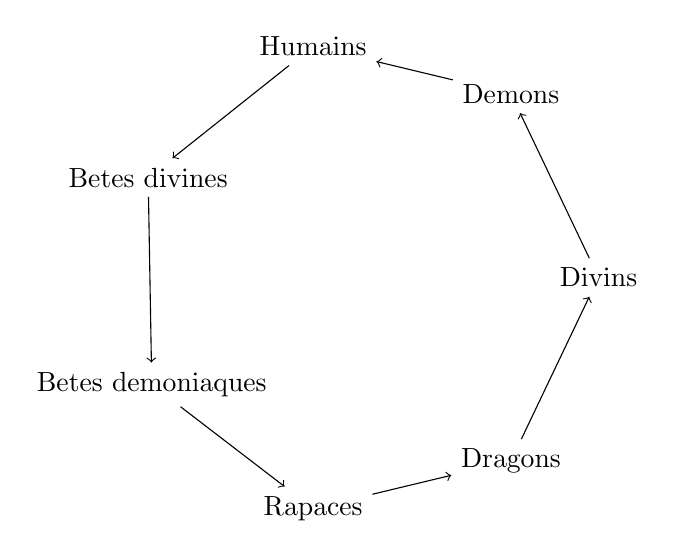
\begin{tikzpicture}[->=stealth]
		\node (Di) at (0:3cm)   [] {Divins};
		\node (De) at (51:3cm)  [] {Demons} edge [<-] (Di);
		\node (Hu) at (102:3cm) [] {Humains} edge [<-] (De);
		\node (BDi) at (155:3cm) [] {Betes divines} edge [<-] (Hu);
		\node (BDe) at (207:3cm) [] {Betes demoniaques} edge [<-] (BDi);
		\node (Ai) at (258:3cm) [] {Rapaces} edge [<-] (BDe);
		\node (Dr) at (309:3cm) [] {Dragons} edge [<-] (Ai);
		\draw[->] (Dr) -- (Di);
	\end{tikzpicture}
\end{center}

\subsection{Les Classes Divins (inverse des secm péchés capitaux)}
	\begin{center}
	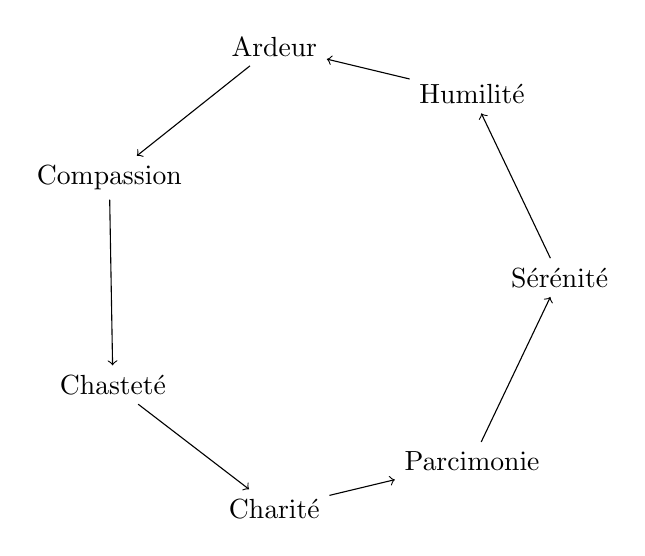
\begin{tikzpicture}
		\node (Se) at (0:3cm) [] {Sérénité};
		\node (Hu) at (51:3cm) [] {Humilité} edge [<-] (Se);
		\node (Ar) at (102:3cm) [] {Ardeur} edge [<-] (Hu);
		\node (Co) at (155:3cm) [] {Compassion} edge [<-] (Ar);
		\node (Cs) at (207:3cm) [] {Chasteté} edge [<-] (Co);
		\node (Cr) at (258:3cm) [] {Charité} edge [<-] (Cs);
		\node (Pa) at (309:3cm) [] {Parcimonie} edge [<-] (Cr);
		\draw[->] (Pa) -- (Se);
	\end{tikzpicture}
	\end{center}

\subsection{Les Classes Démoniaques (les secm péchés capitaux)}
	\begin{center}
	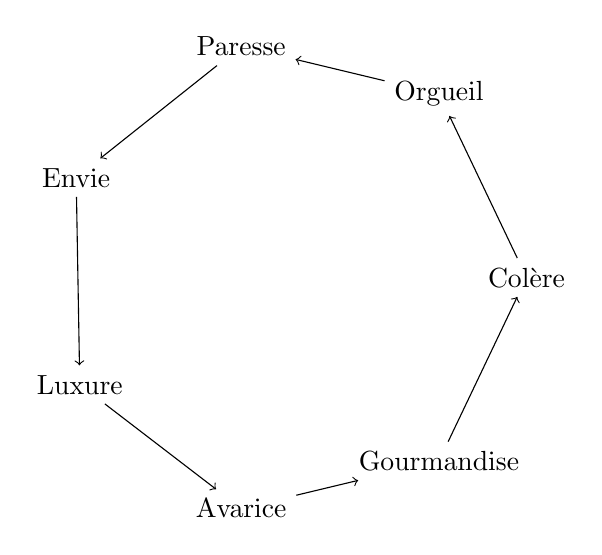
\begin{tikzpicture}[->=stealth]
		\node (Se) at (0:3cm) [] {Colère};
		\node (Hu) at (51:3cm) [] {Orgueil} edge [<-] (Se);
		\node (Ar) at (102:3cm) [] {Paresse} edge [<-] (Hu);
		\node (Co) at (155:3cm) [] {Envie} edge [<-] (Ar);
		\node (Cs) at (207:3cm) [] {Luxure} edge [<-] (Co);
		\node (Cr) at (258:3cm) [] {Avarice} edge [<-] (Cs);
		\node (Pa) at (309:3cm) [] {Gourmandise} edge [<-] (Cr);
		\draw[->] (Pa) -- (Se);
	\end{tikzpicture}
	\end{center}

\subsection{Les Rapaces}
	\begin{center}
		\begin{tikzpicture}[->=stealth]
			\node (Co) at (0:3cm) [] {Chouette};
			\node (Ai) at (51:3cm) [] {Aigle} edge [<-] (Co);
			\node (Fa) at (102:3cm) [] {Faucon} edge [<-] (Ai);
			\node (Se) at (155:3cm) [] {Serpentaire} edge [<-] (Fa);
			\node (Hi) at (207:3cm) [] {Hibou} edge [<-] (Se);
			\node (Ch) at (258:3cm) [] {Condor} edge [<-] (Hi);
			\node (Va) at (309:3cm) [] {Vautour} edge [<-] (Ch);
			\draw[->] (Va) -- (Co);
		\end{tikzpicture}
	\end{center}

\subsection{Humains}
	\begin{center}
		\begin{tikzpicture}[->=stealth]
			\node (Co) at (0:3cm) [] {Epée};
			\node (Ai) at (51:3cm) [] {Sorts} edge [<-] (Co);
			\node (Fa) at (102:3cm) [] {Arts martiaux} edge [<-] (Ai);
			\node (Se) at (155:3cm) [] {Arc} edge [<-] (Fa);
			\node (Hi) at (207:3cm) [] {Fouet} edge [<-] (Se);
			\node (Ch) at (258:3cm) [] {Lance} edge [<-] (Hi);
			\node (Va) at (309:3cm) [] {Marteau} edge [<-] (Ch);
			\draw[->] (Va) -- (Co);
		\end{tikzpicture}
	\end{center}

\subsection{Bêtes Divines}
	\begin{center}
		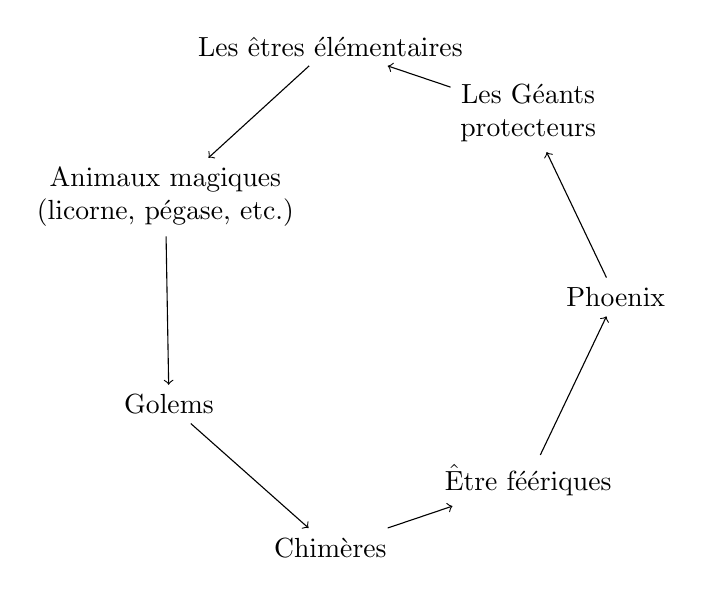
\begin{tikzpicture}[->=stealth]
			\node (Co) at (0:3cm)   [] {Phoenix};
			\node (Ai) at (51:3cm)  [align=center] {Les Géants\\protecteurs} edge [<-] (Co);
			\node (Fa) at (102:3cm) [above] {Les êtres élémentaires} edge [<-] (Ai);
			\node (Se) at (155:3cm) [align=center] {Animaux magiques\\
									  (licorne, pégase, etc.)} edge [<-] (Fa);
			\node (Hi) at (207:3cm) [] {Golems} edge [<-] (Se);
			\node (Ch) at (258:3cm) [below] {Chimères} edge [<-] (Hi);
			\node (Va) at (309:3cm) [] {Être féériques} edge [<-] (Ch);
			\draw[->] (Va) -- (Co);
		\end{tikzpicture}
	\end{center}

\subsection{Bêtes Démoniaques}
	\begin{center}
		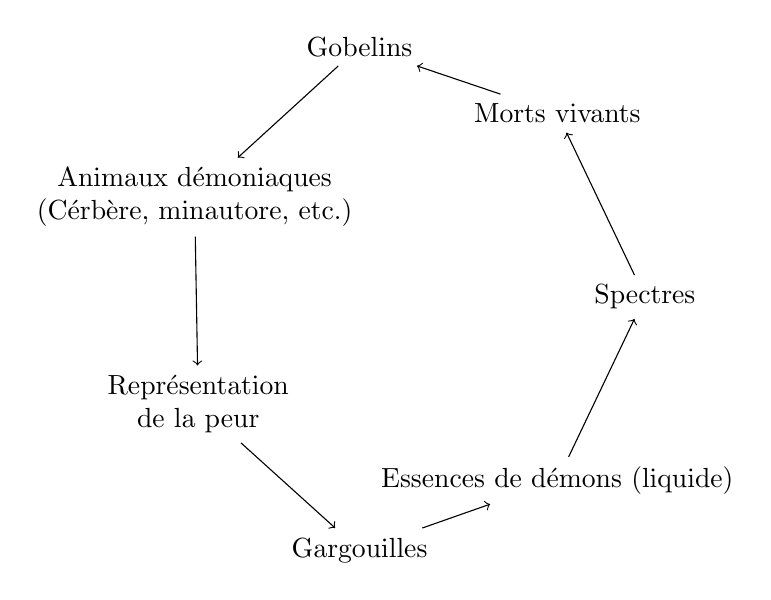
\begin{tikzpicture}[->=stealth]
			\node (Co) at (0:3cm)   [] {Spectres};
			\node (Ai) at (51:3cm)  [align=center] {Morts vivants} edge [<-] (Co);
			\node (Fa) at (102:3cm) [above] {Gobelins} edge [<-] (Ai);
			\node (Se) at (155:3cm) [align=center] {Animaux démoniaques\\
									  (Cérbère, minautore, etc.)} edge [<-] (Fa);
		    \node (Hi) at (207:3cm) [align=center] {Représentation\\de la peur} edge [<-] (Se);
			\node (Ch) at (258:3cm) [below] {Gargouilles} edge [<-] (Hi);
			\node (Va) at (309:3cm) [] {Essences de démons (liquide)} edge [<-] (Ch);
			\draw[->] (Va) -- (Co);
		\end{tikzpicture}
	\end{center}

\subsection{Dragons}
	\begin{center}
		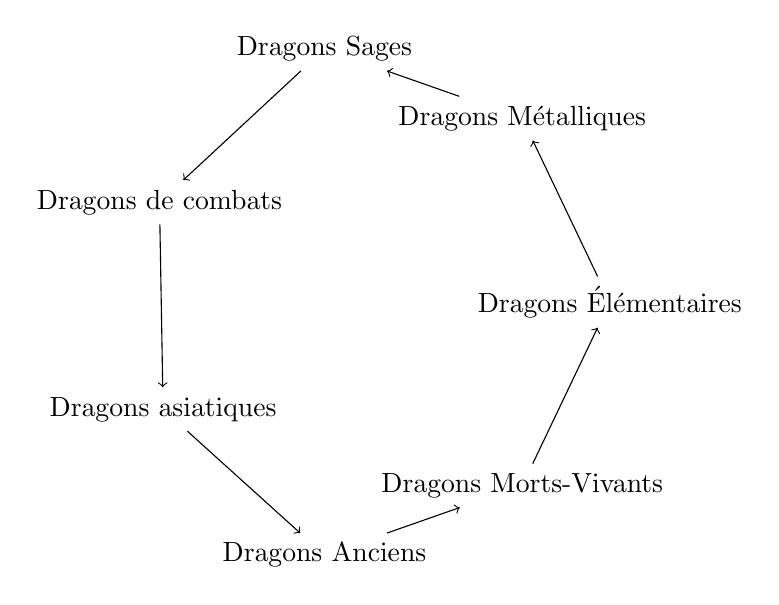
\begin{tikzpicture}
			\node (Co) at (0:3cm)   [] {Dragons Élémentaires};
			\node (Ai) at (51:3cm)  [align=center] {Dragons Métalliques} edge [<-] (Co);
			\node (Fa) at (102:3cm) [above] {Dragons Sages} edge [<-] (Ai);
			\node (Se) at (155:3cm) [align=center] {Dragons de combats} edge [<-] (Fa);
		    \node (Hi) at (207:3cm) [align=center] {Dragons asiatiques} edge [<-] (Se);
			\node (Ch) at (258:3cm) [below] {Dragons Anciens} edge [<-] (Hi);
			\node (Va) at (309:3cm) [] {Dragons Morts-Vivants} edge [<-] (Ch);
			\draw[->] (Va) -- (Co);
		\end{tikzpicture}
	\end{center}

\subsection{Les métaux précieux}
	\begin{center}
		\begin{tikzpicture}
			\node (Co) at (0:3cm)   [] {Adamentium};
			\node (Ai) at (51:3cm)  [align=center] {Platine} edge [<-] (Co);
			\node (Fa) at (102:3cm) [above] {L'or} edge [<-] (Ai);
			\node (Se) at (155:3cm) [align=center] {L'émeraude} edge [<-] (Fa);
		    \node (Hi) at (207:3cm) [align=center] {Le saphir} edge [<-] (Se);
			\node (Ch) at (258:3cm) [below] {Le ruby} edge [<-] (Hi);
			\node (Va) at (309:3cm) [] {Le diamants} edge [<-] (Ch);
			\draw[->] (Va) -- (Co);
		\end{tikzpicture}
	\end{center}

\subsection{Éléments}
	\begin{center}
		\begin{tikzpicture}[->=stealth]
			\node (Co) at (0:3cm) []   {Terre};
			\node (Ai) at (51:3cm) []  {Eau} edge [<-] (Co);
			\node (Fa) at (102:3cm) [] {Feu} edge [<-] (Ai);
			\node (Se) at (155:3cm) [] {Foudre} edge [<-] (Fa);
			\node (Hi) at (207:3cm) [] {Air} edge [<-] (Se);
			\node (Ch) at (258:3cm) [] {Lumières} edge [<-] (Hi);
			\node (Va) at (309:3cm) [] {Ténèbres} edge [<-] (Ch);
			\draw[->] (Va) -- (Co);
		\end{tikzpicture}
	\end{center}

